\PassOptionsToPackage{dvipsnames,table}{xcolor} 
\documentclass{beamer}\usepackage[]{graphicx}\usepackage[]{color}
%% maxwidth is the original width if it is less than linewidth
%% otherwise use linewidth (to make sure the graphics do not exceed the margin)
\makeatletter
\def\maxwidth{ %
  \ifdim\Gin@nat@width>\linewidth
    \linewidth
  \else
    \Gin@nat@width
  \fi
}
\makeatother

\definecolor{fgcolor}{rgb}{0.345, 0.345, 0.345}
\newcommand{\hlnum}[1]{\textcolor[rgb]{0.686,0.059,0.569}{#1}}%
\newcommand{\hlstr}[1]{\textcolor[rgb]{0.192,0.494,0.8}{#1}}%
\newcommand{\hlcom}[1]{\textcolor[rgb]{0.678,0.584,0.686}{\textit{#1}}}%
\newcommand{\hlopt}[1]{\textcolor[rgb]{0,0,0}{#1}}%
\newcommand{\hlstd}[1]{\textcolor[rgb]{0.345,0.345,0.345}{#1}}%
\newcommand{\hlkwa}[1]{\textcolor[rgb]{0.161,0.373,0.58}{\textbf{#1}}}%
\newcommand{\hlkwb}[1]{\textcolor[rgb]{0.69,0.353,0.396}{#1}}%
\newcommand{\hlkwc}[1]{\textcolor[rgb]{0.333,0.667,0.333}{#1}}%
\newcommand{\hlkwd}[1]{\textcolor[rgb]{0.737,0.353,0.396}{\textbf{#1}}}%

\usepackage{framed}
\makeatletter
\newenvironment{kframe}{%
 \def\at@end@of@kframe{}%
 \ifinner\ifhmode%
  \def\at@end@of@kframe{\end{minipage}}%
  \begin{minipage}{\columnwidth}%
 \fi\fi%
 \def\FrameCommand##1{\hskip\@totalleftmargin \hskip-\fboxsep
 \colorbox{shadecolor}{##1}\hskip-\fboxsep
     % There is no \\@totalrightmargin, so:
     \hskip-\linewidth \hskip-\@totalleftmargin \hskip\columnwidth}%
 \MakeFramed {\advance\hsize-\width
   \@totalleftmargin\z@ \linewidth\hsize
   \@setminipage}}%
 {\par\unskip\endMakeFramed%
 \at@end@of@kframe}
\makeatother

\definecolor{shadecolor}{rgb}{.97, .97, .97}
\definecolor{messagecolor}{rgb}{0, 0, 0}
\definecolor{warningcolor}{rgb}{1, 0, 1}
\definecolor{errorcolor}{rgb}{1, 0, 0}
\newenvironment{knitrout}{}{} % an empty environment to be redefined in TeX

\usepackage{alltt}
\usepackage{pgfplots}
\usetikzlibrary{positioning} 
\usepackage[latin1]{inputenc}
\usetheme{Warsaw}

%for drawing, do not need to load tikz in beamer
\usetikzlibrary{snakes}
\usetikzlibrary{shapes,shadows,arrows}
\definecolor{drkgreen}{RGB}{5,102,51}

\usepackage{verbatim}
\usepackage{setspace}
\usepackage{array}

%for math
\usepackage{actuarialangle}
\usepackage{mathptmx}
\usepackage{amsmath, amsfonts}
\usepackage{amsthm, amssymb}
\usepackage[makeroom]{cancel}

\hypersetup{colorlinks=true, linkcolor=white, citecolor=blue, urlcolor=blue, linktocpage=true, breaklinks=true}
\graphicspath{ {./image/}}


\title[How to Use Color and Draw Diagrams in \LaTeX]{Introduction  to Packages \textit{xcolor} and \emph{tikz} \\ How to make an impression with \LaTeX?}
\author{Brian Pham}
\institute{}
\date{February 24, 2014}
\IfFileExists{upquote.sty}{\usepackage{upquote}}{}




\begin{document}


\begin{frame}
\titlepage
\end{frame}

\begin{frame}

\begin{figure}
\resizebox{7.5cm}{!}{
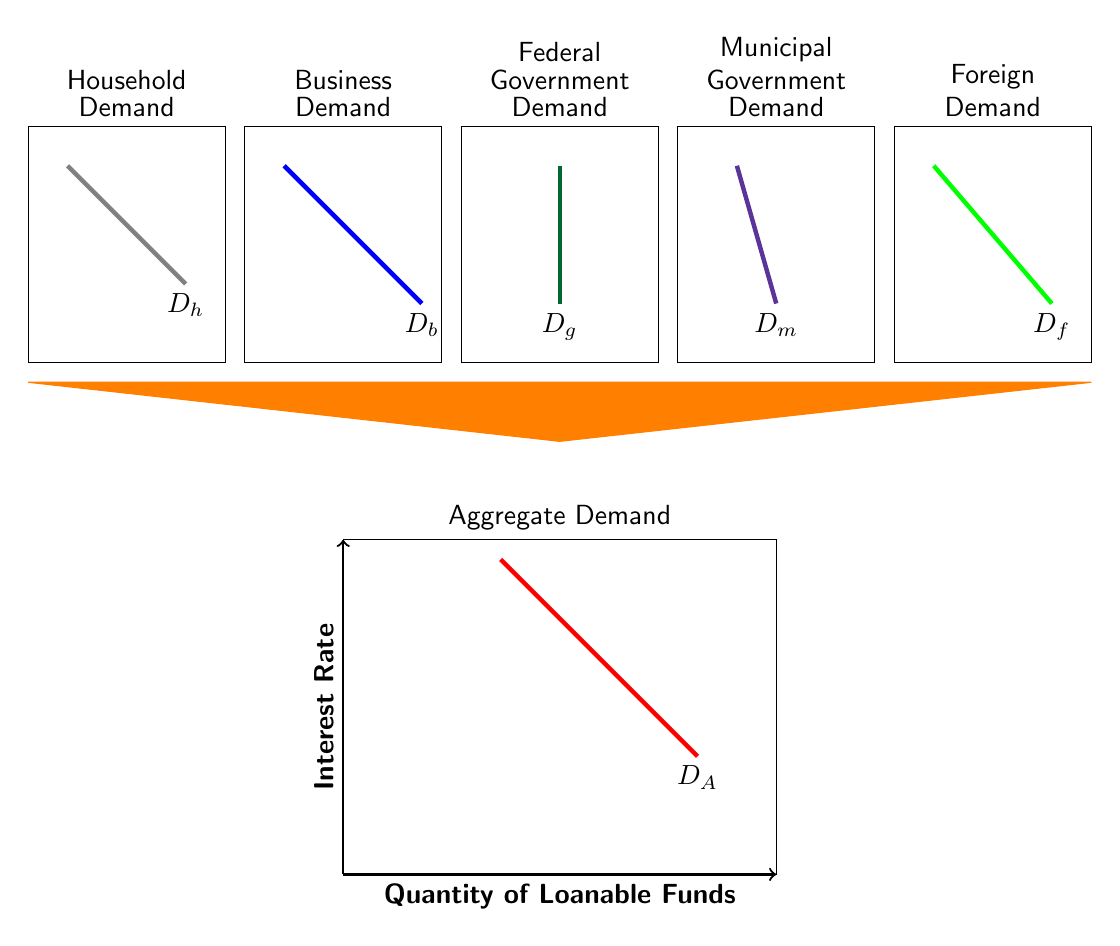
\begin{tikzpicture}
    \draw  (0,0) rectangle (2.5,3) (2.75,0) rectangle (5.25,3) (5.5,0) rectangle (8,3) 
            (8.25,0) rectangle (10.75,3)(11,0) rectangle (13.5,3);
            
     \draw [fill=orange,orange] (0,-.25)--(13.5,-.25)--(6.75,-1)--(0,-.25) ;
     \draw (4,-2.25) rectangle (9.5,-6.5);
     \draw [->, black, thick](4,-6.5)--(4,-2.25);
     \draw [->, black, thick](4,-6.5)--(9.5,-6.5);
     \node [above] at (6.75,-2.25){\textsf{Aggregate Demand}};
     \node [below] at (6.75,-6.5){\textsf{\textbf{Quantity of Loanable Funds}}};
     \node [above,rotate=90] at (4,-4.375){\textsf{\textbf{Interest Rate}}};
     \draw [ultra thick, red] (6,-2.5)--(8.5,-5);
      \node [below] at ((8.5,-5){$D_A$}; 
      
    \draw [ultra thick, gray] (.5,2.5)--(2,1);
    \node [below] at (2,1){$D_h$}; 
    \node [above] at (1.25,3.35){\textsf{Household}};
    \node [above] at (1.25,3){\textsf{Demand}};
    
     \draw [ultra thick, blue] (3.25,2.5)--(5,.75);
    \node [below] at (5,.75){$D_b$};
    \node [above] at (4,3.35){\textsf{Business}};
    \node [above] at (4,3){\textsf{Demand}};
    
    \draw [ultra thick, drkgreen] (6.75,2.5)--(6.75,.75);
    \node [below] at (6.75,.75){$D_g$};
    \node [above] at (6.75,3.7){\textsf{Federal}};
    \node [above] at (6.75,3.35){\textsf{Government}};
    \node [above] at (6.75,3){\textsf{Demand}};
    
    \draw [ultra thick, RoyalPurple] (9,2.5)--(9.5,.75);
    \node [below] at (9.5,.75){$D_m$};
    \node [above] at (9.5,3.7){\textsf{Municipal}};
    \node [above] at (9.5,3.35){\textsf{Government}};
    \node [above] at (9.5,3){\textsf{Demand}};
    
     \draw [ultra thick, green] (11.5,2.5)--(13,.75);
    \node [below] at (13,.75){$D_f$};
    \node [above] at (12.25,3.35){\textsf{Foreign}};
    \node [above] at (12.25,3){\textsf{Demand}};
    
  
\end{tikzpicture}}

\end{figure}
\end{frame}

\begin{frame}
\begin{center}
\renewcommand{\arraystretch}{1.5}
\rowcolors{2}{Turquoise!25}{gray!10}
\resizebox{9cm}{!}{
\begin{tabular}{rlp{10cm}}
\multicolumn{2}{l}{\cellcolor{Turquoise!60}\textsf{\color{white}\textbf{PERSONALITY DIMENSION}}}&\cellcolor{Turquoise!60}\textsf{\color{white}\textbf{CHARACTERISTICS OF A PERSON SCORING POSITIVELY ON THE DIMENSION}}\\
1.&\textbf{\textsf{Extraversion}}&\textsf{Outgoing, talkative, sociable, assertive}\\
2.&\textbf{\textsf{Agreeableness}}&\textsf{Trusting, good-natured, cooperative, softhearted}\\
3.&\textbf{\textsf{Conscientiousness}}&\textsf{Dependable, responsible, achievement oriented, persistent}\\
4.&\textbf{\textsf{Emotional stability}}&\textsf{Relaxed, secure, unworried}\\
5.&\textbf{\textsf{Openness to experience}}&\textsf{Intellectual, imaginative, curious, broad-minded}
\end{tabular}}\end{center}

\pause
\begin{figure}[h]
\centering
\tikzstyle{block} = [draw, rectangle, fill=Lavender, text width=5em, text centered, minimum height=13mm, node distance=4em]
\tikzstyle{block1} = [draw, rectangle, fill=ForestGreen, text width=5em, text centered, minimum height=13mm, node distance=4em]
\tikzstyle{block2} = [draw, rectangle, fill=BlueGreen, text width=5em, text centered,minimum height=13mm, node distance=4em]
\tikzstyle{line} = [draw, -latex', thick,color=black]


\resizebox{8cm}{!}{
\begin{tikzpicture}[x=5,y=5].
\node [block] (ValueSim) {\textsf{Value similarity}};
\node [block, above of=ValueSim, yshift=1em] (Fam) {\textsf{Family values}};

\node [block, below of=ValueSim, yshift=-3em](Congr){\textsf{Value congruence}};
\node [block, below of=Congr, yshift=-1em](work){\textsf{Work value}};
\node [block1, left of=Congr, xshift=-5em, yshift=4em] (Gen) {\textsf{General life values}};

\node [block2, right of =Gen, xshift=14em] (W-Fam) {\textsf{Work-family conflict}};
\node [block2, right of =Gen, xshift=21em] (ValAtt) {\textsf{Value attainment}};
\node [block2, right of =Gen, xshift=28em] (Satis) {\textsf{Job and life satisfaction}};
%arrows
\path [line] (Gen) |-(Fam);
\path [line] (Gen) |- (work);
\path [line] (Fam) -- (ValueSim);
\path [line] (work) -- (Congr);
\path [line] (Congr) --(W-Fam);
\path [line] (ValueSim) --(W-Fam);.
\path [line] (W-Fam) --(ValAtt);
\path [line](ValAtt)--(Satis);
\end{tikzpicture}}
\caption{\footnotesize{A Values Model of Work-Family Conflict}}
\end{figure}
\end{frame}

\begin{frame}
\begin{figure}[!h]
\centering
\tikzstyle{block} = [ draw, rectangle, fill=blue!50, text width=10em, text centered, minimum height=15mm, node distance=5em]
\tikzstyle{block1} = [draw, rectangle, fill=ForestGreen, text width=8em, text centered, minimum height=15mm, node distance=7em]
\tikzstyle{block2} = [draw, rectangle, fill=Fuchsia, text width=10em, text centered,minimum height=25mm, node distance=5em]
\tikzstyle{decision} = [diamond, draw, node distance=12em, fill=RubineRed]
\tikzstyle{line} = [draw, -latex', ultra thick,color=red!50]
\tikzstyle{elli}=[draw, ellipse, fill=red!50,minimum height=8mm, text width=5em, text centered]

\resizebox{7cm}{!}{
\begin{tikzpicture}
\node [block] (MF) {\color{white}\textbf{Mutual Funds}};
\node [block, above of=MF, yshift=1em] (FC) {\color{white}\textbf{Finance Companies}};
\node [decision, left of=FC, xshift=-5em] (SU) {\color{white}\textbf{Surplus Units}};
\node [block, above of=FC, yshift=1em] (DI) {\color{white}\textbf{Depository Institutions (Commercial Banks, Savings Institutions, Credit Unions)}};
\node [block, below of=MF, yshift=-1em](Ins){\color{white}\textbf{Insurance Companies}};
\node [block1, left of=Ins, xshift=-10em] (Holders) {\color{white}\textbf{Policyholders}};
\node [block, below of=Ins, yshift=-1em](PF){\color{white}\textbf{Pension Funds}};
\node [block1, left of=PF, xshift=-10em] (EE) {\color{white}\textbf{Employers and Employees}};
\node [elli, right of=MF, xshift=10em] (DU) {\color{white}\textbf{Deficit Units (Firms. Government Agencies, Some Individuals)}};

%arrows
\path [line] (SU) |-node[yshift=0.755em, xshift=8em] {\color{black}Deposits}(DI);
\path [line] (SU) -- node[yshift=0.75em, xshift=.5em] {\color{black}Purchase} node[yshift=-0.75em, xshift=.5em] {\color{black}Securities}(FC);
\path [line] (SU) |- node[yshift=0.75em, xshift=8em] {\color{black}Purchase} node[yshift=-0.75em, xshift=8em] {\color{black}Shares}(MF);
\path [line] (Holders) -- node[yshift=0.75em, xshift=.5em] {\color{black}Premium}(Ins);
\path [line] (EE) -- node[yshift=0.75em, xshift=.5em] {\color{black}Employee} node[yshift=-0.75em, xshift=.5em] {\color{black}Contributions}(PF);

\path [line] (DI) -|(DU);
\path [line] (FC) -| (DU);
\path [line] (MF) -- (DU);
\path [line] (Ins) -| (DU);
\path [line] (PF) -|(DU);

\end{tikzpicture}}
\caption{
\footnotesize{Comparison of Roles among Financial Institutions}}
\end{figure}
\end{frame}

\begin{frame}

\begin{figure}[h]\begin {center}
\resizebox{8cm}{!}{
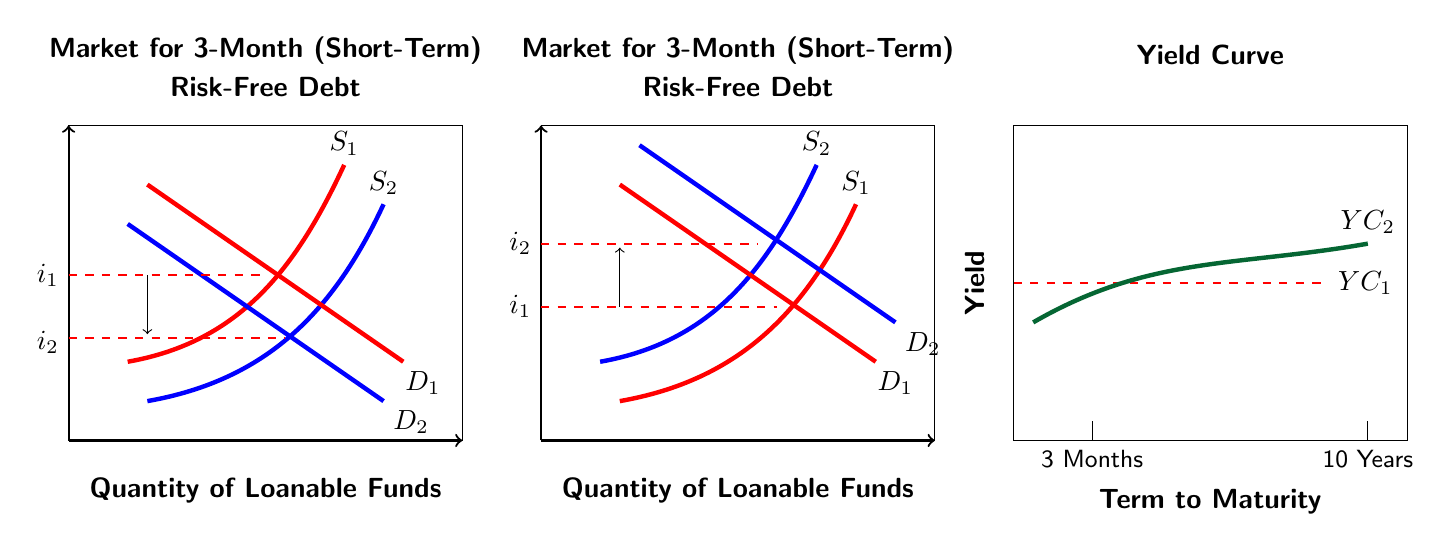
\begin{tikzpicture}
     \draw (0,0) rectangle (5,4);
     \draw [->, black, thick](0,0)--(0,4);
     \draw [->, black, thick](0,0)--(5,0);
     \draw [<-, black](1,1.35)--(1,2.1);
    
     \node [below] at (2.5,-.35){\textsf{\textbf{Quantity of Loanable Funds}}};
     \node [above] at (2.5,4.65){\textsf{\textbf{Market for 3-Month (Short-Term)}}};
     \node [above] at (2.5,4.25){\textsf{\textbf{Risk-Free Debt}}};
     \draw [ultra thick, red] (.75,1) [out=10, in=-115] to  (3.5,3.5);
      \draw [ultra thick, blue] (1,.5) [out=10, in=-115] to  (4,3);
     \draw [ultra thick, blue] (.75,2.75) --  (4,.5);
     \draw [ultra thick, red] (1,3.25) --  (4.25,1);
     
     \draw [thick,dashed,red] (0,1.3) --  (2.75,1.3);
     \draw [thick,dashed,red] (0,2.1) --  (2.5,2.1);
     \node [left] at (0,1.25){$i_2$};
     \node [left] at (0,2.1){$i_1$};
     \node [below] at (4.5,1){$D_{1}$};
     \node [below right] at (4,.5){$D_2$}; 
      \node [above] at (4,3){$S_2$};   
       \node [above] at (3.5,3.5){$S_1$};  
     
     
        \draw (6,0) rectangle (11,4);
     \draw [->, black, thick](6,0)--(6,4);
     \draw [->, black, thick](6,0)--(11,0);
     \draw [->, black](7,1.7)--(7,2.45);
    
     \node [below] at (8.5,-.35){\textsf{\textbf{Quantity of Loanable Funds}}};
     \node [above] at (8.5,4.65){\textsf{\textbf{Market for 3-Month (Short-Term)}}};
     \node [above] at (8.5,4.25){\textsf{\textbf{Risk-Free Debt}}};
     \draw [ultra thick, blue] (6.75,1) [out=10, in=-115] to  (9.5,3.5);
      \draw [ultra thick, red] (7,.5) [out=10, in=-115] to  (10,3);
     \draw [ultra thick, blue] (7.25,3.75) --  (10.5,1.5);
     \draw [ultra thick, red] (7,3.25) --  (10.25,1);
     
     \draw [thick,dashed,red] (6,1.70) --  (9,1.70);
     \draw [thick,dashed,red] (6,2.5) --  (8.75,2.5);
     \node [left] at (6,1.7){$i_1$};
     \node [left] at (6,2.5){$i_2$};
     \node [below] at (10.5,1){$D_{1}$};
     \node [below right] at (10.5,1.5){$D_2$}; 
      \node [above] at (10,3){$S_1$};   
       \node [above] at (9.5,3.5){$S_2$}; 
      
      
       \draw (12,0) rectangle (17,4);
       \draw(13,0)--(13,.25) (16.5,0)--(16.5,.25);
       \draw [thick,dashed,red] (12,2) --  (16,2);
       \node [right] at (16,2){$YC_1$};
       \draw [ultra thick, drkgreen](12.25,1.5)[out=30,in=-170] to (16.5,2.5);
       \node [above] at (16.5,2.5){$YC_2$};
       \node [above,rotate=90] at (11.75,2){\textsf{\textbf{Yield}}};
       \node [above] at (14.5,4.65){\textsf{\textbf{Yield Curve}}};
       \node [below] at (13,0) {\textsf{\small{3 Months}}};
        \node [below] at (16.5,0) {\textsf{\small{10 Years}}};
         \node [below] at (14.5,-.5){\textsf{\textbf{Term to Maturity}}};
\end{tikzpicture}}

\end{center}\end{figure}\vspace*{-.15in}


\begin{figure}[h]
\resizebox{8cm}{!}{
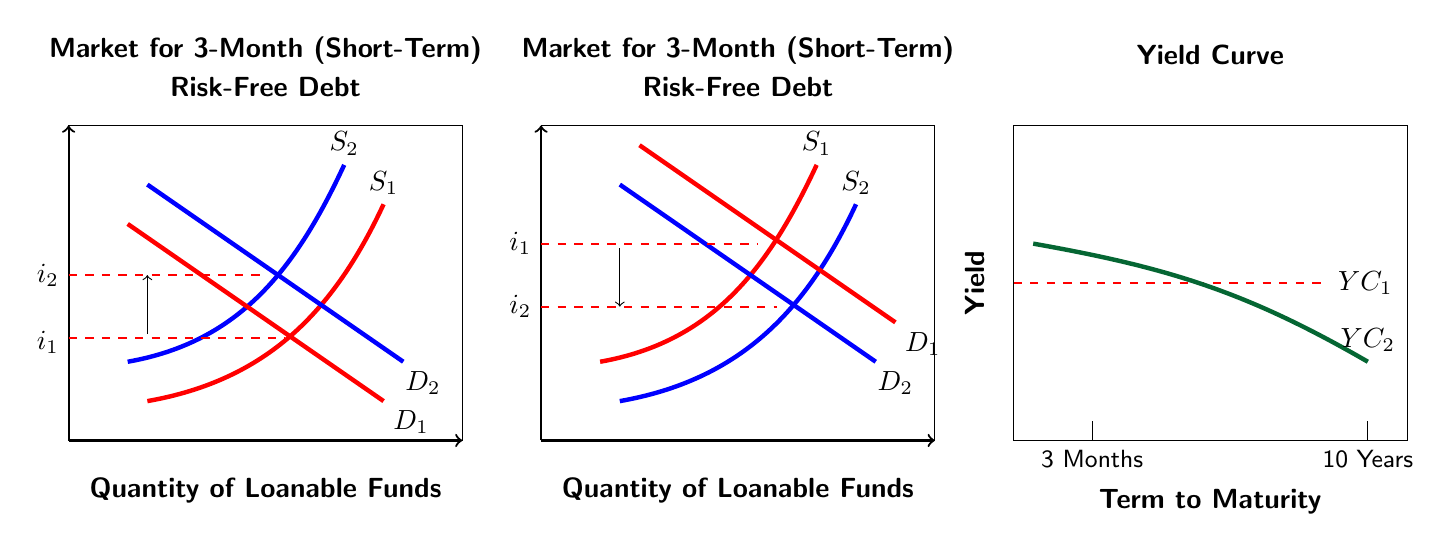
\begin{tikzpicture}
     \draw (0,0) rectangle (5,4);
     \draw [->, black, thick](0,0)--(0,4);
     \draw [->, black, thick](0,0)--(5,0);
     \draw [->, black](1,1.35)--(1,2.1);
    
     \node [below] at (2.5,-.35){\textsf{\textbf{Quantity of Loanable Funds}}};
     \node [above] at (2.5,4.65){\textsf{\textbf{Market for 3-Month (Short-Term)}}};
     \node [above] at (2.5,4.25){\textsf{\textbf{Risk-Free Debt}}};
     \draw [ultra thick, blue] (.75,1) [out=10, in=-115] to  (3.5,3.5);
      \draw [ultra thick, red] (1,.5) [out=10, in=-115] to  (4,3);
     \draw [ultra thick, red] (.75,2.75) --  (4,.5);
     \draw [ultra thick, blue] (1,3.25) --  (4.25,1);
     
     \draw [thick,dashed,red] (0,1.3) --  (2.75,1.3);
     \draw [thick,dashed,red] (0,2.1) --  (2.5,2.1);
     \node [left] at (0,1.25){$i_1$};
     \node [left] at (0,2.1){$i_2$};
     \node [below] at (4.5,1){$D_{2}$};
     \node [below right] at (4,.5){$D_1$}; 
      \node [above] at (4,3){$S_1$};   
       \node [above] at (3.5,3.5){$S_2$};  
     
     
    \draw (6,0) rectangle (11,4);
     \draw [->, black, thick](6,0)--(6,4);
     \draw [->, black, thick](6,0)--(11,0);
     \draw [<-, black](7,1.7)--(7,2.45);
    
     \node [below] at (8.5,-.35){\textsf{\textbf{Quantity of Loanable Funds}}};
     \node [above] at (8.5,4.65){\textsf{\textbf{Market for 3-Month (Short-Term)}}};
     \node [above] at (8.5,4.25){\textsf{\textbf{Risk-Free Debt}}};
     \draw [ultra thick, red] (6.75,1) [out=10, in=-115] to  (9.5,3.5);
      \draw [ultra thick, blue] (7,.5) [out=10, in=-115] to  (10,3);
     \draw [ultra thick, red] (7.25,3.75) --  (10.5,1.5);
     \draw [ultra thick, blue] (7,3.25) --  (10.25,1);
     
     \draw [thick,dashed,red] (6,1.70) --  (9,1.70);
     \draw [thick,dashed,red] (6,2.5) --  (8.75,2.5);
     \node [left] at (6,1.7){$i_2$};
     \node [left] at (6,2.5){$i_1$};
     \node [below] at (10.5,1){$D_{2}$};
     \node [below right] at (10.5,1.5){$D_1$}; 
      \node [above] at (10,3){$S_2$};   
       \node [above] at (9.5,3.5){$S_1$}; 
      
      
       \draw (12,0) rectangle (17,4);
       \draw(13,0)--(13,.25) (16.5,0)--(16.5,.25);
       \draw [thick,dashed,red] (12,2) --  (16,2);
       \node [right] at (16,2){$YC_1$};
       \draw [ultra thick, drkgreen](12.25,2.5)[out=-10,in=150] to (16.5,1);
       \node [above] at (16.5,1){$YC_2$};
       \node [above,rotate=90] at (11.75,2){\textsf{\textbf{Yield}}};
       \node [above] at (14.5,4.65){\textsf{\textbf{Yield Curve}}};
       \node [below] at (13,0) {\textsf{\small{3 Months}}};
        \node [below] at (16.5,0) {\textsf{\small{10 Years}}};
         \node [below] at (14.5,-.5){\textsf{\textbf{Term to Maturity}}};
\end{tikzpicture}}
\caption{\footnotesize{Impact of a Sudden Expectation of Changes Interest Rates}}
\end{figure}

\end{frame}

\begin{frame}[fragile]{Introduction to \emph{\textrm{xcolor}}}

\textrm{The package \emph{xcolor} provides users a variety of choices for colors. \LaTeX comes preloaded with package \emph{color}; however, this package does not give users the flexibility of mixing or defining new color patterns.}

\pause
\textrm{Some examples:}
\begin{itemize}
\pause \item How does a mixture of 40\% green and 90\% yellow look like?

\pause{\footnotesize(Answer: \fcolorbox{black}{green!40}{ \footnotesize{40\%}} + \fcolorbox{black}{yellow!90}{ \footnotesize{90\%}} = \fcolorbox{black}{green!40! yellow!90}{\footnotesize{G40Y90}},\verb=\color{green!40!yellow!90}=)}

\pause \item And how does its complementary color look like?

\pause{\footnotesize(Answer: \fcolorbox{black}{-green!40! yellow!90}{\footnotesize{notG40Y90}}, \verb=\color{-green!40!yellow}=)}

\pause \item How about mixing 3 parts of the last color with 2 parts of its complement and 1 part of red?

\pause{\footnotesize(Answer: $3\times$\fcolorbox{black}{green!40! yellow!90}{\footnotesize{$^{\quad}$}} $+$ $2\times$\fcolorbox{black}{-green!40! yellow!90}{\footnotesize{$^{\quad}$}} $+$ $1\times$\fcolorbox{black}{red}{\footnotesize{$^{\quad}$}} $=$ \fcolorbox{black}{rgb:-green!40!yellow,3;green!40!yellow,2;red,1}{\footnotesize{$^{\quad}$}}, \verb=\color{rgb:-green!40!yellow,3;green!40!yellow,2;red,1}=)}

\end{itemize}
\pause
\footnotesize{For more information, go to \url{http://ftp.math.purdue.edu/mirrors/ctan.org/macros/latex/contrib/xcolor/xcolor.pdf}.
}
\end{frame}

\begin{frame}[fragile]{Implementing \emph{\textrm{xcolor}}}
\textrm{The package \emph{\textrm{xcolor}} needs to be loaded in the preamble. If we want to use the premixed colors the we need to specify the \emph{\textrm{xcolor}} options. For example, the command}  \verb=\usepackage[dvipsnames,table]{xcolor}= \textrm{will enable the use of several premixed colors. \\
\pause
Go to \url{http://en.wikibooks.org/wiki/LaTeX/Colors} to check out these colors and their names.}
\pause
\begin{itemize}
  \item To color text, use \verb=\textcolor{defined-color}{text} =; e.g., \verb=\textcolor{BrickRed}{text}= gives \textcolor{BrickRed}{text}
    \begin{itemize}
       \pause \item Or \verb={\color{defined-color} text} =
   \end{itemize}
    \pause\item Other useful commands:\verb=\colorbox, \fcolorbox =
    \pause\item Create your own color, use \verb=\definecolor{''name''}{''model''}{''color-spec''}=. For example, I created my own Dark Green color by \verb=\definecolor{drkgreen}{RGB}{5,102,51}=.
\end{itemize}
\end{frame}

\begin{frame}[fragile]{Colors in \emph{\textrm{tabular}} environment}

\begin{center}
\renewcommand{\arraystretch}{1.5}
\rowcolors{2}{Turquoise!25}{gray!10}
\resizebox{9cm}{!}{
\begin{tabular}{rlp{10cm}}
\multicolumn{2}{l}{\cellcolor{Turquoise!60}\textsf{\color{white}\textbf{PERSONALITY DIMENSION}}}&\cellcolor{Turquoise!60}\textsf{\color{white}\textbf{CHARACTERISTICS OF A PERSON SCORING POSITIVELY ON THE DIMENSION}}\\
1.&\textbf{\textsf{Extraversion}}&\textsf{Outgoing, talkative, sociable, assertive}\\
2.&\textbf{\textsf{Agreeableness}}&\textsf{Trusting, good-natured, cooperative, softhearted}\\
3.&\textbf{\textsf{Conscientiousness}}&\textsf{Dependable, responsible, achievement oriented, persistent}\\
4.&\textbf{\textsf{Emotional stability}}&\textsf{Relaxed, secure, unworried}\\
5.&\textbf{\textsf{Openness to experience}}&\textsf{Intellectual, imaginative, curious, broad-minded}
\end{tabular}}\end{center}


\pause
\begin{table}\tiny

\begin{tabular}{p{10cm}}
\begin{verbatim}
\begin{table}\sffamily
\renewcommand{\arraystretch}{1.5}
\rowcolors{2}{Turquoise!25}{gray!10}
\resizebox{9cm}{!}{
\begin{tabular}{rlp{10cm}}
\multicolumn{2}{l}{\cellcolor{Turquoise!60}{\color{white}\textbf{PERSONALITY DIMENSION}}}
&\cellcolor{Turquoise!60}{\color{white}\textbf{CHARACTERISTICS OF 
A PERSON SCORING POSITIVELY ON THE DIMENSION}}\\
...
...
\end{tabular}}
\end{table}
\end{verbatim}
\end{tabular}
\end{table}
\end{frame}

\begin{frame}[fragile]{Introduction to \emph{\textrm{tikz}}}
\textrm{\emph{Tikz}} is probably the most comprehensive drawing tool for \LaTeX documents. 
  \begin{itemize}
    \pause\item Challenging $-$ Requires a big learning curve
    \pause\item Point mapping $-$ Requires a good knowledge about geometry
    \pause\item Fun
  \end{itemize}
\pause
The \textrm{\emph{Tikz}} package needs to be loaded in the preamble before we can use it. The usual \textrm{\emph{Tikz}} environment looks like this

\begin{table}\small\vspace{-.25in}
\begin{tabular}{p{4cm}}
\begin{verbatim}
\begin{figure}
  \begin{tikzpicture}
     ...code...
  \end{tikzpicture}
\end{figure}
\end{verbatim}
\end{tabular}
\end{table}
\end{frame}

\begin{frame}[fragile]{\emph{\textrm{Tikz}} $-$ The Basics}


\begin{table}\tiny\rmfamily\vspace{-.25in}
\renewcommand{\arraystretch}{-3}
\begin{tabular}[t]{p{4cm}p{6cm}}
\begin{verbatim}
\begin{tikzpicture}
\draw (0,0) --(3,1);
\end{tikzpicture}
\end{verbatim} 

\begin{center}
\begin{tikzpicture}[scale=.6]
\draw (0,0) --(3,1);
\end{tikzpicture}
\end{center}

& \pause
\begin{verbatim}
\draw (0,0) --(1,2) -- (2,3) -- (1,0);
\draw[help lines] (0,0) grid (2,3);
\end{verbatim} 

\begin{center}
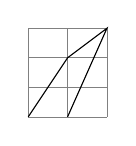
\begin{tikzpicture}[scale=.5, yscale=.75]
\draw[help lines] (0,0) grid (2,3);
\draw (0,0) --(1,2) -- (2,3) -- (1,0);
\end{tikzpicture}
\end{center}
\\\pause

\begin{verbatim}
\draw [ultra thick, blue, fill=orange] 
    (0,0) rectangle (1.5,1);
\draw [red, ultra thick] (3,0.5) 
      circle [radius=0.5];;
\draw [gray] (6,0) arc [radius=1, 
    start angle=45, end angle= 120];
\end{verbatim}

\begin{center}

\begin{tikzpicture}[scale=.75]
\draw [blue,fill=orange] (0,0) rectangle (1.5,1);
\draw [red, ultra thick] (3,0.5) circle [radius=0.5];
\draw [gray] (6,0) arc [radius=1, start angle=45, end angle= 120];
\end{tikzpicture}
\end{center}
&\pause
\begin{verbatim}

\draw [help lines, <->] (0,0) -- (6.5,0);
\draw [help lines, ->] (0,-1.1) -- (0,1.1);
\draw [green,domain=0:2*pi]
    plot (\x, {(sin(\x r)* ln(\x+1))/2});
\draw [red,domain=0:pi] plot (\x, {sin(\x r)});
\draw [blue, domain=pi:2*pi] 
    plot (\x, {cos(\x r)*exp(\x/exp(2*pi))});

\end{verbatim}

\begin{center}
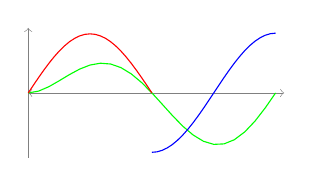
\begin{tikzpicture}[scale=.5, yscale=1.5]
\draw [help lines, <->] (0,0) -- (6.5,0);
\draw [help lines, ->] (0,-1.1) -- (0,1.1);
\draw [green,domain=0:2*pi] plot (\x, {(sin(\x r)* ln(\x+1))/2});
\draw [red,domain=0:pi] plot (\x, {sin(\x r)});
\draw [blue, domain=pi:2*pi] plot (\x, {cos(\x r)*exp(\x/exp(2*pi))});
\end{tikzpicture}
\end{center}
\end{tabular}\vspace{-.25in}

\end{table}
\tiny {For more information, go to \url{http://cremeronline.com/LaTeX/minimaltikz.pdf}.}
\end{frame}


\begin{frame}[fragile]{More Involved Examples}
\textbf{Financial Time Lines}
\begin{center}
\resizebox{9cm}{!}{
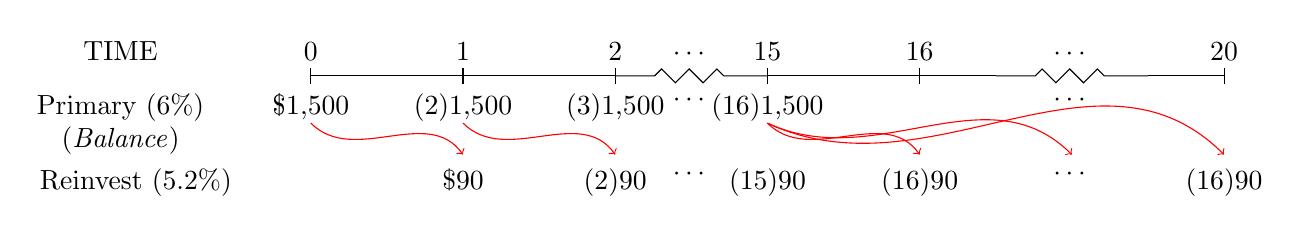
\begin{tikzpicture}[snake=zigzag, line before snake = 5mm, line after snake = 5mm,x=55]

  \draw (1,0) (2,0)-- (3,0)--(4,0)(5,0)--(5.5,0);
  \draw[red,->]  (2,-.6) to [out=-45,in=-235] (3,-1);
  \draw[red,->]  (3,-.6) to [out=-45,in=-235] (4,-1);
  \draw[red,->]  (5,-.6) to [out=-45,in=-235] (6,-1);
  \draw[red,->]  (5,-.6) to [out=-25,in=-225] (7,-1);
  \draw[red,->]  (5,-.6) to [out=-25,in=-225] (8,-1);
       
  \draw[snake] (4,0)--(5,0) (6.5,0)--(7.5,0);   
  \draw (5.5,0)--(6.5,0)(7.5,0)--(8,0);
  \draw  (.75,0) node[left,above=2pt] {TIME};
  \draw  (0.75,0) node[left,below=3pt] {Primary (6\%)};
  \draw  (0.75,0) node[left,below=15pt] {(\textit{Balance})};
  \draw   (.85,0) node[left,below=30pt] {Reinvest (5.2\%)};
        
  \draw (2, 0) node[above=2pt] {0};
  \draw (3, 0) node[above=2pt] {1};
  \draw (4, 0) node[above=2pt] {2};
  \draw (4.5, 0) node[above=2pt] {$\cdots$};
  \draw (5, 0) node[above=2pt] {15};
  \draw (6, 0) node[above=2pt] {16};
  \draw (7, 0) node[above=2pt] {$\cdots$};
  \draw (8, 0) node[above=2pt] {20};
        
  \draw (2, 0) node[below=3pt] {\$1,500};
  \draw (3, 0) node[below=3pt] {(2)1,500};
  \draw (4, 0) node[below=3pt] {(3)1,500};
  \draw (4.5, 0) node[below=3pt] {$\cdots$};
  \draw (5, 0) node[below=3pt] {(16)1,500};      
  \draw (7, 0) node[below=3pt] {$\cdots$};
       
        
  \draw (2, 0) node[below=30pt] {};
  \draw (3, 0) node[below=30pt] {$\$90$};
  \draw (4, 0) node[below=30pt] {$(2)90$};
  \draw (4.5, 0) node[below=30pt] {$\cdots$};
  \draw (5, 0) node[below=30pt] {$(15)90$};
  \draw (6, 0) node[below=30pt] {$(16)90$};
  \draw (7, 0) node[below=30pt] {$\cdots$};
  \draw (8, 0) node[below=30pt] {$(16)90$};       
        
  \draw[] (2,-0.1) -- (2,0.1);
  \draw[] (3,-0.1) -- (3,0.1);
  \draw[] (4,-0.1) -- (4,0.1);
  \draw[] (5,-0.1)  --(5,0.1);
  \draw[] (6,-0.1) -- (6,0.1);
  \draw[] (7,-0.1)  (7,0.1);
  \draw[] (8,-0.1) -- (8,0.1);
   \end{tikzpicture}}
\end{center}

\tiny\begin{verbatim}
\begin{tikzpicture}[snake=zigzag, line before snake = 5mm, line after snake = 5mm,x=55]

  \draw (1,0) (2,0)-- (3,0)--(4,0)(5,0)--(5.5,0);
  \draw[red,->]  (2,-.6) to [out=-45,in=-235] (3,-1);
  \draw[red,->]  (3,-.6) to [out=-45,in=-235] (4,-1);
  \draw[red,->]  (5,-.6) to [out=-45,in=-235] (6,-1);
  \draw[red,->]  (5,-.6) to [out=-25,in=-225] (7,-1);
  \draw[red,->]  (5,-.6) to [out=-25,in=-225] (8,-1);
       
  \draw[snake] (4,0)--(5,0) (6.5,0)--(7.5,0);   
  \draw (5.5,0)--(6.5,0)(7.5,0)--(8,0);
  \draw  (.75,0) node[left,above=2pt] {TIME};
  \draw  (0.75,0) node[left,below=3pt] {Primary (6\%)};
  \draw  (0.75,0) node[left,below=15pt] {(\textit{Balance})};
  \draw   (.85,0) node[left,below=30pt] {Reinvest (5.2\%)};
        
  \draw (2, 0) node[above=2pt] {0};
  \draw (3, 0) node[above=2pt] {1};
  \draw (4, 0) node[above=2pt] {2};
  \draw (4.5, 0) node[above=2pt] {$\cdots$};
  \draw (5, 0) node[above=2pt] {15};
  \draw (6, 0) node[above=2pt] {16};
  \draw (7, 0) node[above=2pt] {$\cdots$};
  \draw (8, 0) node[above=2pt] {20};
\end{verbatim}      
 
\end{frame}

\begin{frame}[fragile]
\begin{center}
\resizebox{9cm}{!}{
\begin{tikzpicture}[snake=zigzag, line before snake = 5mm, line after snake = 5mm,x=55]

  \draw (1,0) (2,0)-- (3,0)--(4,0)(5,0)--(5.5,0);
  \draw[red,->]  (2,-.6) to [out=-45,in=-235] (3,-1);
  \draw[red,->]  (3,-.6) to [out=-45,in=-235] (4,-1);
  \draw[red,->]  (5,-.6) to [out=-45,in=-235] (6,-1);
  \draw[red,->]  (5,-.6) to [out=-25,in=-225] (7,-1);
  \draw[red,->]  (5,-.6) to [out=-25,in=-225] (8,-1);
       
  \draw[snake] (4,0)--(5,0) (6.5,0)--(7.5,0);   
  \draw (5.5,0)--(6.5,0)(7.5,0)--(8,0);
  \draw  (.75,0) node[left,above=2pt] {TIME};
  \draw  (0.75,0) node[left,below=3pt] {Primary (6\%)};
  \draw  (0.75,0) node[left,below=15pt] {(\textit{Balance})};
  \draw   (.85,0) node[left,below=30pt] {Reinvest (5.2\%)};
        
  \draw (2, 0) node[above=2pt] {0};
  \draw (3, 0) node[above=2pt] {1};
  \draw (4, 0) node[above=2pt] {2};
  \draw (4.5, 0) node[above=2pt] {$\cdots$};
  \draw (5, 0) node[above=2pt] {15};
  \draw (6, 0) node[above=2pt] {16};
  \draw (7, 0) node[above=2pt] {$\cdots$};
  \draw (8, 0) node[above=2pt] {20};
        
  \draw (2, 0) node[below=3pt] {\$1,500};
  \draw (3, 0) node[below=3pt] {(2)1,500};
  \draw (4, 0) node[below=3pt] {(3)1,500};
  \draw (4.5, 0) node[below=3pt] {$\cdots$};
  \draw (5, 0) node[below=3pt] {(16)1,500};      
  \draw (7, 0) node[below=3pt] {$\cdots$};
       
        
  \draw (2, 0) node[below=30pt] {};
  \draw (3, 0) node[below=30pt] {$\$90$};
  \draw (4, 0) node[below=30pt] {$(2)90$};
  \draw (4.5, 0) node[below=30pt] {$\cdots$};
  \draw (5, 0) node[below=30pt] {$(15)90$};
  \draw (6, 0) node[below=30pt] {$(16)90$};
  \draw (7, 0) node[below=30pt] {$\cdots$};
  \draw (8, 0) node[below=30pt] {$(16)90$};       
        
  \draw[] (2,-0.1) -- (2,0.1);
  \draw[] (3,-0.1) -- (3,0.1);
  \draw[] (4,-0.1) -- (4,0.1);
  \draw[] (5,-0.1)  --(5,0.1);
  \draw[] (6,-0.1) -- (6,0.1);
  \draw[] (7,-0.1)  (7,0.1);
  \draw[] (8,-0.1) -- (8,0.1);
   \end{tikzpicture}}
\end{center}

\tiny\begin{verbatim}
  \draw (2, 0) node[below=3pt] {\$1,500};
  \draw (3, 0) node[below=3pt] {(2)1,500};
  \draw (4, 0) node[below=3pt] {(3)1,500};
  \draw (4.5, 0) node[below=3pt] {$\cdots$};
  \draw (5, 0) node[below=3pt] {(16)1,500};      
  \draw (7, 0) node[below=3pt] {$\cdots$};
       
        
  \draw (2, 0) node[below=30pt] {};
  \draw (3, 0) node[below=30pt] {$\$90$};
  \draw (4, 0) node[below=30pt] {$(2)90$};
  \draw (4.5, 0) node[below=30pt] {$\cdots$};
  \draw (5, 0) node[below=30pt] {$(15)90$};
  \draw (6, 0) node[below=30pt] {$(16)90$};
  \draw (7, 0) node[below=30pt] {$\cdots$};
  \draw (8, 0) node[below=30pt] {$(16)90$};       
        
  \draw[] (2,-0.1) -- (2,0.1);
  \draw[] (3,-0.1) -- (3,0.1);
  \draw[] (4,-0.1) -- (4,0.1);
  \draw[] (5,-0.1)  --(5,0.1);
  \draw[] (6,-0.1) -- (6,0.1);
  \draw[] (7,-0.1)  (7,0.1);
  \draw[] (8,-0.1) -- (8,0.1);
\end{tikzpicture}
\end{verbatim}   
\end{frame}

\begin{frame}[fragile]
\textbf{\large{Diagrams in \textrm{\emph{Tikz}}}}

\begin{figure}[!h]
\centering
\tikzstyle{block} = [ draw, rectangle, fill=blue!50, text width=10em, text centered, minimum 
                      height=15mm, node distance=5em]
\tikzstyle{block1} = [draw, rectangle, fill=ForestGreen, text width=8em, text centered,        
                      minimum height=15mm, node distance=7em]
\tikzstyle{block2} = [draw, rectangle, fill=Fuchsia, text width=10em, text centered,minimum 
                      height=25mm, node distance=5em]
\tikzstyle{decision} = [diamond, draw, node distance=12em, fill=RubineRed]
\tikzstyle{line} = [draw, -latex', ultra thick,color=red!50]
\tikzstyle{elli}=[draw, ellipse, fill=red!50,minimum height=8mm, text width=5em, text centered]
\resizebox{6cm}{!}{
\begin{tikzpicture}
\node [block] (MF) {\color{white}\textbf{Mutual Funds}};
\node [block, above of=MF, yshift=1em] (FC) {\color{white}\textbf{Finance Companies}};
\node [decision, left of=FC, xshift=-5em] (SU) {\color{white}\textbf{Surplus Units}};
\node [block, above of=FC, yshift=1em] (DI) {\color{white}\textbf{Depository Institutions
          (Commercial Banks, Savings Institutions, Credit Unions)}};
\node [block, below of=MF, yshift=-1em](Ins){\color{white}\textbf{Insurance Companies}};
\node [block1, left of=Ins, xshift=-10em] (Holders) {\color{white}\textbf{Policyholders}};
\node [block, below of=Ins, yshift=-1em](PF){\color{white}\textbf{Pension Funds}};
\node [block1, left of=PF, xshift=-10em] (EE) {\color{white}\textbf{Employers and Employees}};
\node [elli, right of=MF, xshift=10em] (DU) {\color{white}\textbf{Deficit Units (Firms.
            Government Agencies, Some Individuals)}};

\path [line] (SU) |-node[yshift=0.755em, xshift=8em] {\color{black}Deposits}(DI);
\path [line] (SU) -- node[yshift=0.75em, xshift=.5em] {\color{black}Purchase} 
                  node[yshift=-0.75em, xshift=.5em] {\color{black}Securities}(FC);
\path [line] (SU) |- node[yshift=0.75em, xshift=8em] {\color{black}Purchase} 
                  node[yshift=-0.75em, xshift=8em] {\color{black}Shares}(MF);
\path [line] (Holders) -- node[yshift=0.75em, xshift=.5em] {\color{black}Premium}(Ins);
\path [line] (EE) -- node[yshift=0.75em, xshift=.5em] {\color{black}Employee} 
                node[yshift=-0.75em, xshift=.5em] {\color{black}Contributions}(PF);

\path [line] (DI) -|(DU);
\path [line] (FC) -|(DU);
\path [line] (MF) --(DU);
\path [line] (Ins) -|(DU);
\path [line] (PF) -|(DU);

\end{tikzpicture}}
\end{figure}

\tiny\begin{verbatim}
\begin{figure}[!h]
\centering
\tikzstyle{block} = [ draw, rectangle, fill=blue!50, text width=10em, text centered, minimum 
                      height=15mm, node distance=5em]
\tikzstyle{block1} = [draw, rectangle, fill=ForestGreen, text width=8em, text centered,        
                      minimum height=15mm, node distance=7em]
\tikzstyle{block2} = [draw, rectangle, fill=Fuchsia, text width=10em, text centered,minimum 
                      height=25mm, node distance=5em]
\tikzstyle{decision} = [diamond, draw, node distance=12em, fill=RubineRed]
\tikzstyle{line} = [draw, -latex', ultra thick,color=red!50]
\tikzstyle{elli}=[draw, ellipse, fill=red!50,minimum height=8mm, text width=5em, text centered]
\end{verbatim}
\end{frame}



\begin{frame}[fragile]
\tiny\begin{verbatim}
\resizebox{7cm}{!}{
\begin{tikzpicture}
\node [block] (MF) {\color{white}\textbf{Mutual Funds}};
\node [block, above of=MF, yshift=1em] (FC) {\color{white}\textbf{Finance Companies}};
\node [decision, left of=FC, xshift=-5em] (SU) {\color{white}\textbf{Surplus Units}};
\node [block, above of=FC, yshift=1em] (DI) {\color{white}\textbf{Depository Institutions
          (Commercial Banks, Savings Institutions, Credit Unions)}};
\node [block, below of=MF, yshift=-1em](Ins){\color{white}\textbf{Insurance Companies}};
\node [block1, left of=Ins, xshift=-10em] (Holders) {\color{white}\textbf{Policyholders}};
\node [block, below of=Ins, yshift=-1em](PF){\color{white}\textbf{Pension Funds}};
\node [block1, left of=PF, xshift=-10em] (EE) {\color{white}\textbf{Employers and Employees}};
\node [elli, right of=MF, xshift=10em] (DU) {\color{white}\textbf{Deficit Units (Firms.
            Government Agencies, Some Individuals)}};

\path [line] (SU) |-node[yshift=0.755em, xshift=8em] {\color{black}Deposits}(DI);
\path [line] (SU) -- node[yshift=0.75em, xshift=.5em] {\color{black}Purchase} 
                  node[yshift=-0.75em, xshift=.5em] {\color{black}Securities}(FC);
\path [line] (SU) |- node[yshift=0.75em, xshift=8em] {\color{black}Purchase} 
                  node[yshift=-0.75em, xshift=8em] {\color{black}Shares}(MF);
\path [line] (Holders) -- node[yshift=0.75em, xshift=.5em] {\color{black}Premium}(Ins);
\path [line] (EE) -- node[yshift=0.75em, xshift=.5em] {\color{black}Employee} 
                node[yshift=-0.75em, xshift=.5em] {\color{black}Contributions}(PF);

\path [line] (DI) -|(DU);
\path [line] (FC) -|(DU);
\path [line] (MF) --(DU);
\path [line] (Ins) -|(DU);
\path [line] (PF) -|(DU);

\end{tikzpicture}}
\end{figure}
\end{verbatim}\vspace*{-.25in}
Check this out \url{http://elishapeterson.wikidot.com/tikz:diagrams}.
\end{frame}

\begin{frame}{Take-Home Challenge}

\begin{figure}[h]
     \centering
      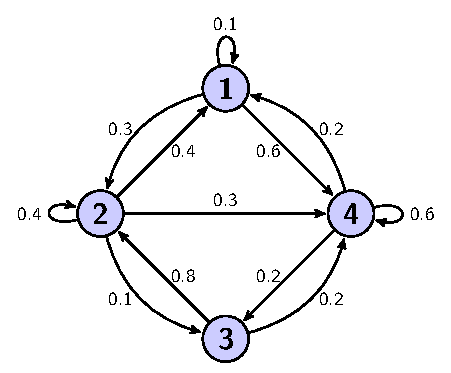
\includegraphics[scale=.6]{graph.pdf}
     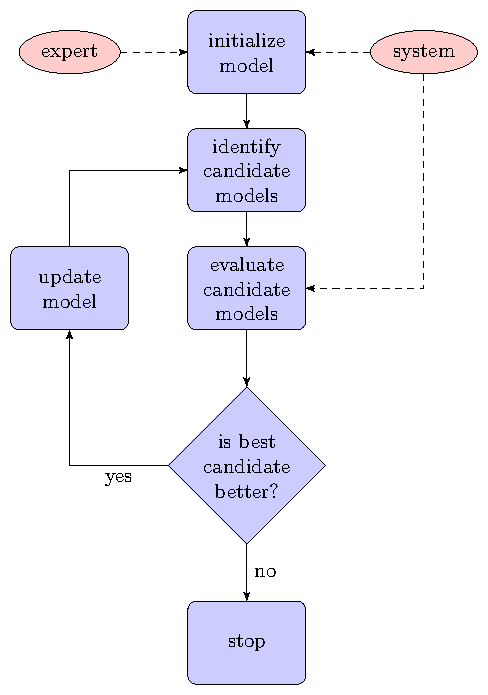
\includegraphics[scale=.6]{SimpleFlowChart.pdf}
    
     \label{fig:SimpleFlowChart}
\end{figure}

\end{frame}
\end{document}
